\chapter{Introduction}

Traditionally, electricity has been generated in centralised power plants.
It is conditioned, stepped up and fed into High-Voltage (HV) transmission networks.
These HV networks span over large distances and even allow the exchange of electricity amongst different nations.
Once the electricity has been transmitted to the area of demand, it is stepped down to Medium-Voltage (MV) levels.
At this level it can either be delivered to primary or secondary consumers (e.g. larger factory complexes or superstores) or it is transmitted to local substations.
Those substations lower the voltage to a statutory level of 230V (which is considered Low-Voltage (LV)) so it can be delivered to urban or rural households and customers.
This so called radial network was designed to transmit energy outwards consumers at the network edge, i.e. away from centralised generators and towards lower voltage levels.
Yet with the transition of energy generation towards renewable energy sources and energy consumers' behaviours becoming less predictable, this power flow concept does no longer hold.

In this chapter, an introduction into the incentives for the current trend in energy supply and demand is presented. The associated issues with these trends are addressed and arising technical problems are explained. Finally, a high level summary of potential solutions is presented before delving into a detailed literature review of current technologies and research.

\section{Current trend in energy systems}

% Basic introduction into the energy trend
Electric energy has become a vital commodity for the uninterrupted functioning of today's society.
In the UK, two aspects can be identified that have accelerated the increase in electricity demand.
For one, political incentives to strengthen the county's independence from oil, coal and gas.
A result would be the electrification of e.g. railroads and household appliances, where electricity is replacing fossil fuels that were required as diesel propellant, and gas or oil that were needed for central heating systems.
In addition to the political incentive, socio-environmental ambitions to reduce $\text{CO}_2$ emissions to counter climate change played an important role in the uptake of electricity.
This ambition to reach the EU target of a 20\% reduction in emissions by 2020 has sparked the subsidisation and installation of Low-Carbon-Technologies (LTCs).

Focusing on electric LTCs, these consist of passive and active energy solutions.
Passive solutions include replacement of old technologies with modern substitutes, e.g. light bulb replacement or upgrading heating systems.
These technologies aim to reduce the consumption of electric energy by improving the device's efficiency.
Active solutions on the other hand, reduce the consumption of electric energy by locally generating electricity.
These solution consist of Photo-Voltaic (PV) installations, diesel generators or wind turbines.
To some degree, Energy Storage Solutions (ESSs) and Electric Vehicles (EVs) can be included into the pool of active solutions since they may be used to actively coordinate the flow and consumption of energy.

\begin{figure}[htb]
	\centering
	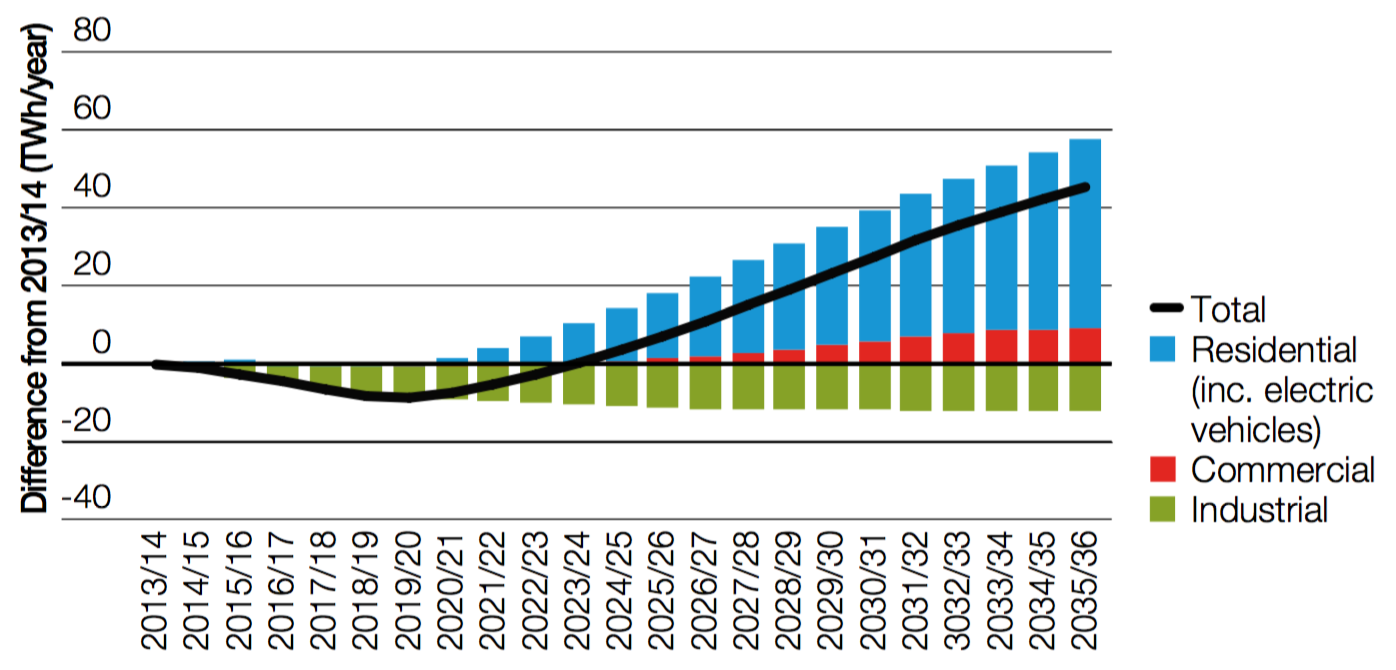
\includegraphics[width=0.8\textwidth]{_introduction/gone-green-power-change-2014-onwards}
	\caption{Power consumption expectation based on ``gone-green'' FES2015 scenario in
comparison to 2013/14 by type (excluding losses) (figure from \cite{FES2015})}
	\label{fig-gone-green-power-change}
\end{figure}

Nonetheless and despite the foreseen uptake of LTCs the Future Energy Scenario (FES), which was produced by National Grid, has identified and predicts an ongoing increase in electricity demand \cite{FES2015}.
This trend is depicted in the graph in Figure \ref{fig-gone-green-power-change}, which has been taken from the FES 2015.
Additionally, with Distributed Energy Resources (DER) the demand for electric energy becomes highly variable, e.g. due to changes in cloud cover or fluctuation in wind speed.
Both the increase in electricity demand as well as the associated amplification of energy variability put significant strain on the current power distribution network.

\section{Issues arising from the energy transition}

% Issues that are foreseen to arise due to current energy trends
The strain put onto the power distribution network may push asset utilisation beyond its limits.
In some cases, exceeding physical limits is virtually impossible.
For instance, substation transformers are usually derated for their deployment environment and protected by circuit breaking fuses or autoreclosers.
Here, if a high current event causes a breaker to open, power loss is only a temporary problem.
On the other hand, if a cable's thermal limits is exceeded for a prolonged time, degradation and insulation failure may occur.
In this case prolonged loss of power delivery may cause significant and sometimes punishable outages.

Whilst these scenarios describe the worst case, voltage deviation and system imbalance are more common occurrences.
The European statutory voltage is 230V with a tolerance band of +10\% -6\% - i.e. 253V and 216.2V.


\section{Technical challenges and barriers to entry}

% Main Problems that have been identified

\section{Proposed solutions and research motivation}

% Transition into possible solutions that are elaborated in the literature review